\documentclass[conference]{IEEEtran}
\IEEEoverridecommandlockouts

\usepackage{cite}
\usepackage{amsmath,amssymb,amsfonts}
\usepackage{graphicx}
\usepackage{textcomp}
\usepackage{xcolor}
\usepackage{booktabs}
\usepackage{url}
\usepackage{tikz}
\usetikzlibrary{positioning,arrows.meta}

\newcommand{\Glight}{G_{\mathit{light}}}
\newcommand{\Gsafe}{G_{\mathrm{safe}}}
\newcommand{\Bg}{B_g}
\newcommand{\DIRECT}{\textsc{direct}}
\newcommand{\STRONG}{\textsc{strong}}
\newcommand{\REJECT}{\textsc{reject}}

\begin{document}

\title{Safety as a Schedulable Resource: Budget-Aware Admission Control for Multi-Tenant LLM Gateways}

\author{\IEEEauthorblockN{Taixing Bi}
\IEEEauthorblockA{\textit{Independent Researcher}\\
New York, NY, USA\\
taixingbijob@gmail.com}}

\maketitle

\begin{abstract}
Enterprise large language model (LLM) gateways can use a lightweight risk estimator to decide whether an incoming request requires a stronger, more expensive safety check before it reaches a generation model. Existing risk-based routing treats this decision purely as a per-request classification problem: is this request risky enough to warrant a strong guardrail? This framing ignores that the strong guardrail is itself a bounded shared resource, constrained by third-party API cost, per-tenant policy, and organizational safety budgets. We argue that strong safety enforcement should instead be treated as a schedulable resource in multi-tenant LLM gateways, alongside compute and queueing capacity. We present a safety admission controller that jointly considers request risk, tenant policy, available safety budget, queue load, and per-request deadlines, and that enforces a fail-closed invariant: a request whose policy mandates a strong check either receives that check or is rejected early, and is never silently passed through ungated. We characterize the lightweight risk estimator on a frozen, validated benchmark of approximately 1.9K prompts spanning four risk classes, and externally on XSTest and WildGuardTest. Using the resulting frozen risk scores, we then evaluate the admission controller itself across multi-tenant contention, dynamic safety demand, fail-open overload, and deadline-aware rejection, and show that tenant-aware scheduling raises strong-check coverage for a minority sensitive tenant from 29.9\% to 65.5\% at a 90:10 tenant mix, and lowers that tenant's unsafe admission rate (e.g., 0.242 to 0.175 at 70:30); that safety-resource exhaustion can occur independently of changes in aggregate offered load as the risky-request fraction rises from 5\% to 50\% under constant total request-per-second (RPS); that at $1.5\Bg$ offered demand, fail-open policies bypass 57\% of policy-required strong checks and raise the unsafe admission rate from 0.051 to 0.611 for only a 0.017~RPS gain in Safe SLO-Goodput, with bypass reaching 62\% across the swept range; and that deadline-aware early rejection reduces strong-guardrail calls from 39 to 29 with unchanged Safe SLO-Goodput, while cutting safety-stage P95 latency from roughly 2002~ms to 178~ms. These results position guardrail capacity as a first-class scheduling target rather than an afterthought of risk classification.
\end{abstract}

\begin{IEEEkeywords}
LLM gateway, admission control, guardrails, multi-tenant systems, safety-resource scheduling, overload control
\end{IEEEkeywords}

\section{Introduction}

Enterprise deployments of large language models increasingly sit behind a gateway that mediates traffic from many tenants toward one or more backend generation models. To keep latency and cost manageable, a gateway can use a lightweight risk estimator---a small classifier such as a distilled sentence encoder---to score each incoming request and decide whether it warrants a stronger, more expensive safety check, for example a managed guardrail service, before being forwarded to generation~\cite{inan2023llamaguard,rebedea2023nemo,aws_applyguardrail}. This pattern reduces the question of request safety to a single per-request decision: is this request risky enough to need a strong guardrail?

That framing is incomplete. The strong guardrail is not a free, infinitely available function call. In practice it is a bounded shared resource: it has a cost per invocation, it may be subject to a third-party rate limit, and an organization may impose an explicit budget on how much strong-guardrail traffic it is willing to pay for or route through a given provider in a given window. When many tenants share one gateway, and each tenant may carry a different safety policy and a different sensitivity to risk, the interesting systems question is no longer just ``is this request risky'' but rather: \emph{when multiple tenants compete for a bounded strong-guardrail budget under dynamic safety demand, how should the gateway allocate safety checks while respecting tenant policy and latency deadlines?}

This paper answers that question by treating strong-guardrail capacity as a first-class, schedulable resource, analogous to how modern serving systems treat GPU or queueing capacity~\cite{sheng2024fairness,sun2024llumnix,zhong2024distserve,agrawal2024sarathi}. We design a safety admission controller that sits between the lightweight risk estimator and the strong guardrail, and that makes a joint decision based on request risk, tenant policy, remaining safety budget, current queue and load state, and the request's safety-stage deadline. The controller preserves a fail-closed invariant throughout: whenever tenant policy requires a strong check, the request either receives that check if capacity allows, or is rejected early if it cannot be completed in time---it is never silently forwarded to the generation model without the required check.

This paper makes the following contributions:
\begin{itemize}
\item \textbf{Safety capacity as a first-class gateway resource.} We separate physical provider capacity for a strong guardrail from a gateway-controlled safety budget, and study how limited strong-check capacity should be allocated across concurrent tenants and traffic conditions.
\item \textbf{Tenant-aware safety admission control.} We show that the same risk score can warrant different actions for different tenants, and we design a scheduler that reserves scarce strong-check capacity for more sensitive tenants rather than treating all requests identically.
\item \textbf{Deadline-aware, fail-closed admission.} We show that requests which require a strong check but cannot complete it before their safety-stage deadline should be rejected early rather than queued indefinitely or, worse, allowed to bypass the check.
\item \textbf{Empirical evidence of safety-resource exhaustion.} We show experimentally that the safety subsystem of a gateway can become overloaded even when total request throughput is held constant, purely because the fraction of risky requests in the traffic mix increases.
\end{itemize}

\section{Related Work}

\subsection{Guardrails and Safety Enforcement}

Safety research has developed learned guard models, moderation datasets, and benchmarks for identifying unsafe prompts, unsafe responses, jailbreaks, and over-refusal. Llama Guard provides an input/output safeguard model~\cite{inan2023llamaguard}; WildGuard broadens moderation across harmfulness, jailbreak, and refusal detection~\cite{han2024wildguard}; XSTest targets exaggerated safety behavior~\cite{rottger2024xstest}; and AEGIS2.0 provides a broad safety-risk taxonomy and guardrail dataset~\cite{ghosh2025aegis2}. Runtime frameworks such as NeMo Guardrails expose programmable enforcement rails~\cite{rebedea2023nemo}, while managed services such as Amazon Bedrock ApplyGuardrail provide an external policy-enforcement API~\cite{aws_applyguardrail}. These systems primarily study what should be blocked or how a safety policy is enforced; they do not formulate the allocation of policy-required strong checks as a shared, budget-constrained resource across competing tenants.

\subsection{Cost-Aware Routing and Cascades}

A separate line of work reduces inference cost by routing requests among models or cascades. FrugalGPT adaptively combines model calls under cost--quality trade-offs~\cite{chen2024frugalgpt}, while RouteLLM learns per-request routing between stronger and weaker LLMs from preference data~\cite{ong2025routellm}. Their decision variable is which generation model or cascade should serve a request. Closer to our setting, recent guardrail work has explored cascaded detector architectures that selectively invoke a second-stage detector to improve moderation accuracy and computational efficiency~\cite{nagireddy2025cascade}. Such work studies \emph{when} to escalate safety processing to a specialized second-stage detector, but does not model contention for bounded second-stage capacity. Our setting is different: tenant policy may make a strong safety check mandatory, so the controller instead addresses \emph{how scarce, already-triggered} strong-check capacity should be allocated across competing tenants under a bounded budget and per-request deadlines, preserving a fail-closed constraint rather than trading safety enforcement away for lower cost.

\subsection{LLM Serving and Resource Scheduling}

LLM serving systems study fairness, dynamic scheduling, tail latency, and SLO-constrained goodput for inference resources. Fairness in Serving Large Language Models introduces token-aware fair scheduling across clients~\cite{sheng2024fairness}; Llumnix dynamically reschedules requests for load balance, priority, and SLO isolation~\cite{sun2024llumnix}; DistServe optimizes serving capacity under TTFT and TPOT constraints~\cite{zhong2024distserve}; and Sarathi-Serve studies the throughput--latency trade-off in batched LLM inference~\cite{agrawal2024sarathi}. More broadly, Dominant Resource Fairness formalizes fair allocation of shared resources~\cite{ghodsi2011drf}, and tail-latency work motivates deadline-aware control in large-scale services~\cite{dean2013tail}. We borrow these systems concepts but apply them to a different resource and constraint set: strong-guardrail invocations have their own budget and queue, tenants have heterogeneous safety policies, and policy-required checks cannot be silently bypassed under overload.

\section{System Design}
\label{sec:design}

Fig.~\ref{fig:arch} shows the overall gateway architecture. An incoming request first passes through a lightweight risk estimator, $\Glight$, implemented as a MiniLM-L12-H384-based estimator~\cite{wang2020minilm} that produces a continuous risk score $q(x)$ rather than a hard label. This score is combined with the requesting tenant's safety policy to determine the request's safety requirement: whether a strong check is optional, required, or waivable under specific conditions.

\begin{figure}[t]
\centering
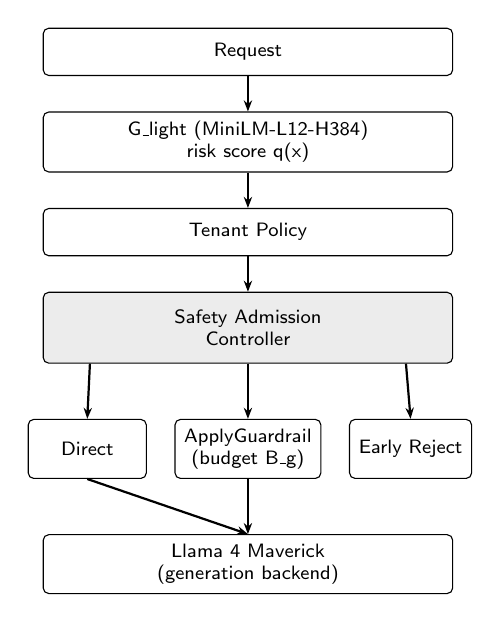
\begin{tikzpicture}[
  font=\sffamily\scriptsize,
  box/.style={draw, rounded corners=2pt, minimum height=0.6cm, align=center},
  wide/.style={box, minimum width=5.2cm},
  small/.style={box, minimum width=1.5cm, minimum height=0.75cm},
  arr/.style={-{Stealth[length=4pt]}, thick},
  node distance=0.45cm
]
\node[wide] (req) {Request};
\node[wide, below=of req] (glight) {G\_light (MiniLM-L12-H384)\\risk score q(x)};
\node[wide, below=of glight] (policy) {Tenant Policy};
\node[wide, below=of policy, fill=gray!15, minimum height=0.9cm] (sac) {Safety Admission\\Controller};
\node[small, below=0.7cm of sac] (ag) {ApplyGuardrail\\(budget B\_g)};
\node[small, left=0.35cm of ag] (direct) {Direct};
\node[small, right=0.35cm of ag] (rej) {Early Reject};
\node[wide, below=0.7cm of ag] (llm) {Llama 4 Maverick\\(generation backend)};
\draw[arr] (req) -- (glight);
\draw[arr] (glight) -- (policy);
\draw[arr] (policy) -- (sac);
\draw[arr] (sac.south west) ++(0.6,0) -- (direct.north);
\draw[arr] (sac) -- (ag);
\draw[arr] (sac.south east) ++(-0.6,0) -- (rej.north);
\draw[arr] (direct.south) -- (llm.north);
\draw[arr] (ag) -- (llm);
\end{tikzpicture}
\caption{Gateway architecture: lightweight risk estimator, tenant policy, safety admission controller, bounded strong-guardrail budget, and fail-closed routing to direct pass-through, ApplyGuardrail, or early rejection.}
\label{fig:arch}
\end{figure}

The Safety Admission Controller then makes the routing decision. It has three possible outcomes: direct forwarding to the generation model when no strong check is required or policy allows a waiver; routing to the strong guardrail---in our deployment, the managed Amazon Bedrock ApplyGuardrail API~\cite{aws_applyguardrail}---when capacity within the bounded safety budget $\Bg$ is available; or early rejection when the request requires a strong check but the controller determines that the check cannot be completed before the request's safety-stage deadline, or that insufficient $\Bg$ token-bucket capacity is available. Only requests that pass the strong guardrail, or that are exempted by policy, are forwarded to the generation backend, in our setup a managed Llama 4 Maverick endpoint.

We distinguish the gateway-controlled budget $\Bg$ from the provider's physical service capacity. $\Bg$ is an organizational invocation budget enforced by the gateway; provider throughput or rate limits can impose additional constraints, but are not assumed to equal $\Bg$.

The controller's admission decision is a function of five inputs: (i)~the request's risk score from $\Glight$; (ii)~the requesting tenant's policy, which may mandate, waive, or conditionally require a strong check; (iii)~the currently available fraction of the safety budget $\Bg$; (iv)~the gateway's current queue depth and load; and (v)~the request's remaining time budget before its safety-stage deadline expires.

\subsection{Fail-Closed Invariant}

The controller enforces a single non-negotiable invariant: if tenant policy requires a strong check for a given request, then that request is resolved in exactly one of two ways---it receives the strong check if capacity is available, or it is rejected early if the check cannot be completed safely within the request's deadline. The controller never silently bypasses a policy-required guardrail to preserve throughput or reduce latency. This invariant is what distinguishes the design from throughput-first admission control: under overload, the system sheds load rather than weakening safety guarantees.

\subsection{Tenant-Aware Scheduling}

Because tenants may declare different safety sensitivity, an identical risk score $q(x)$ can imply different actions depending on which tenant issued the request. The scheduler therefore reserves a configurable share of strong-guardrail capacity for higher-sensitivity tenants rather than serving all tenants on a first-come, first-served or purely load-aware basis, which would let a high-volume, low-sensitivity tenant crowd out a low-volume, high-sensitivity tenant's access to required strong checks.

\subsection{Formalization}
\label{sec:formal}

We formalize the admission rule to make the controller's contract precise and reproducible. For request $i$ from tenant $t_i$ with risk score $q_i = \Glight(x_i)$, let
\begin{equation}
r_i = f(q_i, \pi_{t_i}) \in \{0, 1\}
\end{equation}
indicate whether tenant $t_i$'s policy $\pi_{t_i}$ requires a strong check for this request ($r_i = 1$) given its risk score. The controller assigns an action $a_i \in \{\DIRECT, \STRONG, \REJECT\}$. The fail-closed invariant is the constraint
\begin{equation}
r_i = 1 \implies a_i \in \{\STRONG, \REJECT\},
\end{equation}
i.e.\ a policy-required check is never resolved by \DIRECT{} forwarding. Our implementation enforces the strong-check budget with parallel token buckets rather than a single global one: a shared bucket refills at rate $\Bg(1 - \sum_c \rho_c)$ and each reserved sensitivity class $c$ has its own bucket refilling at rate $\rho_c \Bg$, every bucket capped at capacity $b$ ($b = 1$ check in our experiments). Because the per-bucket rates sum to exactly $\Bg$, the long-run strong-check rate is conserved at $\Bg$; however, since the shared bucket and each reserved-class bucket can independently hold up to $b$ tokens, the aggregate instantaneous burst is $(1+C)b$ rather than $b$, where $C$ is the number of reserved classes. Over any measurement window $W$, the controller admits at most
\begin{equation}
\sum_{i \in W} \mathbf{1}[a_i = \STRONG] \;\le\; \Bg\, T_W + (1+C)b,
\end{equation}
where $\Bg$ is the gateway-controlled strong-check rate budget (in checks per unit time; Section~\ref{sec:setup}) and $T_W$ is the duration of window $W$. In the two-tenant configuration used in our experiments (Section~\ref{sec:setup}), only the sensitive tenant carries a reservation ($C = 1$), giving an aggregate bound of $\Bg T_W + 2b$. Unused reservation in a class's bucket may be fully borrowed by another tenant once the reserving tenant is idle (no waiting or in-flight requests) --- our implementation applies no additional fractional cap beyond each bucket's own capacity $b$ --- so idle reserved capacity is not wasted, while a class's reservation cannot be pre-empted while that tenant is active. Finally, request $i$ is assigned $a_i = \REJECT$ instead of \STRONG{} whenever the controller's estimate of remaining queue wait plus strong-guardrail service time would exceed $i$'s remaining safety-stage deadline, or whenever insufficient token-bucket capacity is available; otherwise $a_i = \STRONG$ when $r_i = 1$, and $a_i = \DIRECT$ when $r_i = 0$ or policy grants a waiver.

\section{Metrics}
\label{sec:metrics}

The primary performance metric is Safe SLO-Goodput, a safety-constrained analogue of SLO-oriented serving goodput~\cite{zhong2024distserve}: the rate of requests that are simultaneously policy-compliant, ground-truth safe, served, and completed within their deadline:
\begin{equation}
\Gsafe = \frac{N(\text{policy-compliant} \!\wedge\! \text{safe} \!\wedge\! \text{served} \!\wedge\! \text{deadline met})}{T}
\end{equation}
where $N(\cdot)$ counts qualifying requests over a measurement window of duration $T$, and ground-truth safety is determined by the frozen benchmark labels rather than by the strong guardrail's own decision. Rejected requests may preserve policy compliance but do not contribute to $\Gsafe$ because they are not served. We report four supporting metrics alongside Safe SLO-Goodput, reported in the tables most relevant to each experiment: Unsafe Admission Rate (UAR), the fraction of ground-truth unsafe requests that are admitted to the generation backend, $\mathrm{UAR} = N(\text{unsafe} \wedge \text{admitted}) / N(\text{unsafe})$, which we decompose into admissions caused by $\Glight$ false negatives (routed \DIRECT{} below threshold), strong-guardrail misses, and scheduler bypass; Required-Strong Coverage, the fraction of policy-required strong checks that were actually performed; Policy Bypass Rate, the fraction of policy-required checks that were silently skipped; and safety-stage P95 latency. Unless stated otherwise, the deadline used in E1--E6 is the safety-stage / controller-path deadline (scheduler wait plus strong-guardrail latency); it is not a measured user-facing end-to-end generation SLO.

\section{Experimental Setup}
\label{sec:setup}

\subsection{Benchmark Construction}

We follow a generate-validate-freeze-replay methodology consistent with our prior guardrail evaluation work. Approximately 500 seed prompts are transformed into four risk classes: S0 (clear-safe), S1 (borderline-safe), S2 (direct-unsafe), and S3 (adversarial-unsafe). After validation, the frozen benchmark contains roughly 1.9K prompts. We additionally evaluate against two external benchmarks, XSTest~\cite{rottger2024xstest} and WildGuardTest~\cite{han2024wildguard}, to check that findings are not artifacts of our own prompt-generation process. E0a shows clear score separation on the frozen benchmark for binary safe/unsafe discrimination (S0--S1 as safe-negative, S2--S3 as unsafe-positive): AUROC 0.986, and transfers to the external sets with AUROC 0.811 on XSTest and 0.876 on WildGuardTest; full per-set precision/recall curves are reported in the artifact. Throughout, the MiniLM-based estimator $\Glight$ is used only as the gateway's risk-scoring component; it is never treated as ground truth for whether a prompt is actually safe or unsafe, which is instead determined by the frozen benchmark labels and the external test sets.

Each E1--E6 condition was repeated five times; we report the median across repetitions with the interquartile range [P25, P75] where space permits, and give ground-truth-unsafe counts pooled over repetitions alongside UAR.\footnote{Code, configurations, guardrail policy definition, E0 characterization results, and full per-repetition results: \url{https://github.com/taixingbi/guardrail-admission-control}.} The strong guardrail is a published (non-draft) Amazon Bedrock guardrail version with content filters (hate, insults, sexual, violence, misconduct) at high strength and prompt-attack detection on input, created from the released policy file; every strong-routed request in E1--E6 records the guardrail's verdict, and runs abort if a call returns none.\footnote{The E0b--E6 numbers in this version come from a complete rerun against a guardrail re-created from the same released policy file in a new account, after we found that an earlier campaign had been run with an unset guardrail identifier and therefore never executed the strong check. $\Glight$ scores (E0a) and the generation-backend characterization (E0c) do not depend on the guardrail and are unchanged.} Unless otherwise stated, the main experiments use a frozen, gateway-controlled aggregate safety budget of $\Bg = 0.4$ strong checks/s, implemented using the parallel token-bucket allocation described in Section~\ref{sec:formal}, with each bucket capped at one check. This is an organizational budget, not the provider's physical ApplyGuardrail capacity: E0b separately measures the provider's raw ApplyGuardrail throughput at approximately 101.7~RPS at concurrency 16 (P50/P95 141/231~ms), more than two orders of magnitude above $\Bg$, with zero throttling up to concurrency 16 and 0.1\% at 32; this makes provider-side throttling an unlikely explanation for the safety-resource pressure studied in E1--E6, which instead arises from the gateway-controlled budget by design.

\textbf{Implementation parameters.} The tenant configuration used in E1--E6 fixes a policy threshold $\tau$ (request requires a strong check when $q(x) \ge \tau$) and a safety-stage deadline (SLO) per tenant class: the majority tenant uses $\tau{=}0.75$ and a 600~ms deadline, and the sensitive tenant uses a lower threshold $\tau{=}0.40$ (routing more of its traffic to a strong check) and an 800~ms deadline. The sensitive tenant's reserved share is $\rho{=}0.4$ (40\% of $\Bg$); the majority tenant draws from the remaining shared pool. We fix $\rho = 0.4$ once, before the E2 tenant-mix sweep, and do not retune it across mixes. $\Bg$ here models an organizational safety-spend quota rather than a service-latency capacity limit, so the 600--800~ms deadlines should be read against queueing and strong-guardrail service time under that quota, not against $\Bg$'s refill interval directly. E1 and E3--E6 run the majority tenant only, retaining its $\tau$ and deadline from the same fixed configuration; E2 additionally introduces the sensitive tenant to study multi-tenant contention. We do not retune $\tau$ or the deadlines across experiments.

\textbf{Baselines.} We compare the proposed controller against three policies that share the same $\Bg$ token bucket and never bypass a required check. \emph{Always-Strong} requires a strong check for every request, ignoring $q(x)$; it rejects requests whose deadline cannot be met and otherwise queues when the budget is exhausted. \emph{Risk-only} requires a strong check when $q(x) \ge 0.5$ (a single global threshold, no tenant policy) and rejects when no token is available, with no deadline reasoning. \emph{Load-aware} uses the same global threshold, rejects early when the estimated queue wait plus strong-check time exceeds the deadline, and otherwise queues, sharing capacity first-come, first-served across tenants (hence in proportion to volume). The proposed controller adds tenant-specific thresholds, per-tenant reservations, and rejection rather than queueing when no token is available.

\subsection{Experiment Sequence}

We run three characterization experiments before the main study: E0a characterizes the MiniLM risk estimator's score distribution and separability across the four risk classes; E0b characterizes the latency and throughput of the managed ApplyGuardrail-style strong check in isolation; and E0c characterizes the latency and throughput of the Llama 4 Maverick generation backend in isolation. These establish baseline per-component behavior before the admission controller is introduced.

To isolate scheduling effects from estimator and generation-backend variability, E1--E6 replay the frozen risk scores $q(x)$ produced during E0a rather than re-running $\Glight$ live, while still invoking the strong guardrail (ApplyGuardrail) live; the generation backend is not placed on the hot path of these experiments. We separately run an end-to-end check (proposed controller, $1.0\Bg$, 40~s) with frozen $q(x)$, the live strong guardrail, and the live Maverick backend on the hot path: user-perceived end-to-end latency is P50/P95 555/703~ms, Safe SLO-Goodput is 1.775~RPS at the 600~ms deadline, 70\% of admitted requests meet it, and 0 of 17 ground-truth unsafe requests reach generation.

The main study consists of six experiments. E1 (static safety-budget pressure) measures Safe SLO-Goodput and UAR as offered strong-check demand is held at $0.5$, $1.0$, and $1.5\Bg$. E2 (multi-tenant contention) measures how strong-check coverage is distributed across tenants of different sensitivity under a fixed budget and varying tenant traffic mixes. E3 (dynamic safety demand) measures system behavior as the risky-request fraction changes over time within a session. E4 (safety-resource exhaustion) holds total gateway RPS constant while varying the suspicious-request fraction, isolating safety-budget pressure from changes in aggregate offered load. E5 (fail-open vs.\ fail-closed) compares the fail-closed controller against a fail-open baseline that bypasses required checks under budget pressure. E6 (deadline / early-rejection ablation) compares the full controller against a variant with early rejection disabled. E1--E4 compare all four policies; E5 and E6 vary the proposed controller only.

\section{Results}

\subsection{Baselines Under Static and Dynamic Load (E1, E3)}

\begin{table}[t]
\caption{Baselines at $1.0\Bg$ Static Demand (E1) and Under a Dynamic Mix (E3); Median [P25, P75] over 5 Reps, UAR Counts Pooled}
\label{tab:e1e3}
\centering
\scriptsize
\setlength{\tabcolsep}{3pt}
\begin{tabular}{lcccc}
\toprule
 & \multicolumn{2}{c}{\textbf{E1 ($1.0\Bg$)}} & \multicolumn{2}{c}{\textbf{E3 (dynamic)}} \\
\cmidrule(lr){2-3}\cmidrule(lr){4-5}
\textbf{Policy} & $\boldsymbol{\Gsafe}$ & \textbf{UAR} & $\boldsymbol{\Gsafe}$ & \textbf{UAR} \\
\midrule
Always-Strong & 0.18 [0.15, 0.20] & 0/76 & 0.17 [0.17, 0.18] & 1/874 \\
Risk-only & 2.55 [2.53, 2.58] & 5/84 & 2.59 [2.57, 2.60] & 32/816 \\
Load-aware & 2.48 [2.45, 2.48] & 6/93 & 2.60 [2.58, 2.60] & 39/810 \\
Proposed & 2.53 [2.48, 2.63] & 5/79 & \textbf{2.64} [2.62, 2.65] & 34/816 \\
\bottomrule
\end{tabular}
\end{table}

Table~\ref{tab:e1e3} compares the four policies. Always-Strong spends the entire budget on checks that are mostly unnecessary (only 6--24\% of its strong-check occupancy is on requests with $q(x) \ge \tau$) and, because each live check takes $\approx$190~ms against a 0.4~checks/s budget, rejects 93--95\% of all traffic; its UAR of zero is bought by refusing almost every request, and its Safe SLO-Goodput is roughly $14\times$ lower than any selective policy. The three selective policies are statistically close under static demand (E1: Proposed 2.70, 2.53, 2.40 vs.\ Risk-only 2.68, 2.55, 2.35 at $0.5$, $1.0$, $1.5\Bg$). Under the dynamic mix of E3, in which offered strong demand moves $0.5 \to 0.9 \to 1.5 \to 0.6\Bg$ over 480~s, Proposed attains the highest Safe SLO-Goodput and lowest reject rate (0.117 vs.\ 0.130--0.136); the gap is concentrated in the $1.5\Bg$ overload phase (2.46 [2.36, 2.52] vs.\ 2.33 for both Risk-only and Load-aware), where it also starves fewer required checks (36 vs.\ 46). The strong guardrail let through no examined unsafe request in E1 and at most 3 per policy across all E3 repetitions, so the residual UAR of the selective policies (0.04--0.05 in E3) consists almost entirely of $\Glight$ false negatives.

\subsection{Tenant Isolation (E2)}

Table~\ref{tab:e2} shows strong-check coverage for a minority sensitive tenant under two scheduling policies as the tenant mix is varied from 90:10 (majority:sensitive) down to 30:70. Under load-aware scheduling, which allocates strong-guardrail capacity in proportion to per-tenant request volume, the sensitive tenant's coverage falls as its share of traffic shrinks, dropping to 29.9\% when it represents only 10\% of total traffic. Tenant-aware scheduling, which reserves capacity for higher-sensitivity tenants regardless of volume, raises coverage to 65.5\% at the same 90:10 mix, and continues to dominate load-aware coverage across every mix we tested, though the gap narrows as the sensitive tenant's own share of traffic grows. This result shows that a purely load-proportional allocation of a shared safety resource systematically disadvantages low-volume, high-sensitivity tenants across the full range of tenant mixes, not only at the most favorable operating point, and that an explicit tenant-aware reservation policy is necessary to correct this. The extra coverage also reduces the sensitive tenant's unsafe admission rate $\mathrm{UAR}_B$: tenant-aware scheduling admits 0.175, 0.140, and 0.122 of that tenant's ground-truth unsafe requests at 70:30, 50:50, and 30:70, versus 0.242, 0.232, and 0.206 under load-aware scheduling, with non-overlapping interquartile ranges; at 90:10 the difference (0.222 vs.\ 0.231) is within run-to-run noise. Part of this gain comes from the sensitive tenant's lower threshold ($\tau{=}0.40$) rather than from the reservation alone; the risk-only baseline, which shares neither, has the highest $\mathrm{UAR}_B$ (0.231--0.294).

\begin{table}[t]
\caption{Sensitive-Tenant Strong-Check Coverage (Pooled over 5 Reps) and Unsafe Admission Rate $\mathrm{UAR}_B$ (Median [P25, P75]) Across Tenant Mixes}
\label{tab:e2}
\centering
\scriptsize
\setlength{\tabcolsep}{3pt}
\begin{tabular}{lcccc}
\toprule
 & \multicolumn{2}{c}{\textbf{Coverage}} & \multicolumn{2}{c}{$\mathbf{UAR}_B$} \\
\cmidrule(lr){2-3}\cmidrule(lr){4-5}
\textbf{Mix} & \textbf{Load-Aw.} & \textbf{Tenant-Aw.} & \textbf{Load-Aw.} & \textbf{Tenant-Aw.} \\
\midrule
90:10 & 29.9\% & 65.5\% & 0.23 [0.16, 0.24] & 0.22 [0.13, 0.25] \\
70:30 & 27.1\% & 40.3\% & 0.24 [0.22, 0.27] & 0.18 [0.15, 0.18] \\
50:50 & 25.6\% & 30.9\% & 0.23 [0.21, 0.26] & 0.14 [0.14, 0.18] \\
30:70 & 22.0\% & 25.2\% & 0.21 [0.20, 0.23] & 0.12 [0.10, 0.14] \\
\bottomrule
\end{tabular}
\end{table}

\begin{table}[t]
\caption{Safety-Resource Exhaustion Under Constant Gateway Load (E4, Proposed; Median over 5 Reps)}
\label{tab:e4}
\centering
\begin{tabular}{ccccc}
\toprule
\textbf{Suspicious} & \textbf{Gateway} & \textbf{Strong} & $\boldsymbol{\Gsafe}$ & \textbf{Req.-Strong} \\
\textbf{Mix} & \textbf{RPS} & \textbf{Demand} & & \textbf{Coverage} \\
\midrule
5\%  & 3.01 & $0.38\Bg$ & 2.817 & 0.67 \\
50\% & 3.01 & $3.76\Bg$ & 1.478 & 0.23 \\
5\%  & 3.01 & $0.38\Bg$ & 2.850 & 0.72 \\
\bottomrule
\end{tabular}
\end{table}

\subsection{Safety-Resource Exhaustion (E4)}

We hold total gateway RPS constant at 3.01 and vary only the fraction of suspicious requests in the traffic mix from approximately 5\% to 50\% and back to 5\%. Table~\ref{tab:e4} reports offered strong-guardrail demand (relative to the safety budget $\Bg$), Safe SLO-Goodput, and Required-Strong Coverage (Section~\ref{sec:metrics}) at each operating point. As the suspicious fraction rises from 5\% to 50\%, offered strong-guardrail demand rises from $0.38\Bg$ to $3.76\Bg$---nearly a $10\times$ increase---while Safe SLO-Goodput falls from 2.817 [2.800, 2.850] to 1.478 [1.461, 1.550] and Required-Strong Coverage drops from 0.67 to 0.23, even though total gateway offered load remains fixed at 3.01~RPS throughout. This isolates safety-budget pressure from changes in aggregate offered request rate; because the generation backend is not on the hot path of this experiment (Section~\ref{sec:setup}), we do not directly measure Maverick-side inference load here, but the fixed offered RPS rules out increasing aggregate request volume as the driver of the observed degradation. Returning the suspicious fraction to 5\% recovers Safe SLO-Goodput to 2.850. This demonstrates that the safety subsystem can become an independent bottleneck on system throughput, distinct from and not explained by aggregate request volume---a failure mode that a purely volume-based admission controller would not detect. The exhaustion is a property of the workload, not of one policy: in the 50\% phase all three selective policies are statistically tied (1.478--1.494~RPS, overlapping IQRs), and Always-Strong falls to 0.083. Over the whole run Proposed has the highest Safe SLO-Goodput (2.257 vs.\ 2.229 Load-aware, 2.183 Risk-only) but a slightly higher UAR (0.059 vs.\ 0.044--0.048), so E4 does not show a safety advantage for any selective policy.

\subsection{Fail-Closed vs. Fail-Open (E5)}

Table~\ref{tab:e5} compares the fail-closed controller against a fail-open baseline that, under safety-budget pressure, silently forwards requests to generation without the policy-required strong check rather than rejecting them. At $1.5\Bg$ offered demand, fail-open raises Safe SLO-Goodput by only 0.017~RPS (2.333 to 2.350) while bypassing 57\% of policy-required strong checks and raising the Unsafe Admission Rate twelvefold, from 0.051 (11 of 201 unsafe requests, all $\Glight$ false negatives) to 0.611 (108 of 177). At $2.0\Bg$ the pattern repeats: +0.067~RPS (2.200 to 2.267), 62\% bypass, and UAR 0.095 to 0.636. The $\Glight$-attributable component of UAR is the same in both modes (0.05--0.10); essentially the entire increase is scheduler-induced bypass ($\mathrm{UAR}_{\text{bypass}} = 0.53$--$0.59$), which the fail-closed invariant eliminates by construction. Weakening mandatory checks under overload is therefore a poor systems trade-off even when evaluated purely on goodput: at most a 3\% goodput gain for roughly $7$--$12\times$ more unsafe admissions.

\begin{table}[t]
\caption{Fail-Closed vs.\ Fail-Open (E5, Proposed; Median [P25, P75] over 5 Reps, UAR Counts Pooled)}
\label{tab:e5}
\centering
\footnotesize
\setlength{\tabcolsep}{3pt}
\begin{tabular}{llccc}
\toprule
\textbf{Demand} & \textbf{Mode} & $\boldsymbol{\Gsafe}$ & \textbf{UAR} & \textbf{Bypass} \\
\midrule
$1.5\Bg$ & Fail-closed & 2.33 [2.20, 2.33] & 0.051 (11/201) & 0 \\
         & Fail-open   & 2.35 [2.35, 2.43] & 0.611 (108/177) & 0.57 \\
$2.0\Bg$ & Fail-closed & 2.20 [2.20, 2.22] & 0.095 (20/226) & 0 \\
         & Fail-open   & 2.27 [2.25, 2.28] & 0.636 (138/215) & 0.62 \\
\bottomrule
\end{tabular}
\end{table}

\begin{table}[t]
\caption{Effect of Disabling Deadline-Aware Early Rejection (E6, $1.5\Bg$; Median [P25, P75] over 5 Reps; Safety-Stage P95)}
\label{tab:e6}
\centering
\footnotesize
\setlength{\tabcolsep}{3pt}
\begin{tabular}{lccc}
\toprule
\textbf{Variant} & $\boldsymbol{\Gsafe}$ & \textbf{Strong Calls} & \textbf{P95 (ms)} \\
\midrule
Full & 2.46 [2.36, 2.52] & 29 [27, 30] & 178 [178, 179] \\
No early rej. & 2.46 [2.36, 2.52] & 39 [38, 41] & 2002 [2002, 2002] \\
\bottomrule
\end{tabular}
\end{table}

\subsection{Deadline-Aware Early Rejection (E6)}

Table~\ref{tab:e6} compares the full controller against a variant with early rejection disabled, so that requests requiring a strong check are always queued rather than rejected when they cannot meet their deadline. Disabling early rejection performs 34\% more strong-check work (29 to 39 calls over the measured window) with identical Safe SLO-Goodput, UAR (0.041), and reject rate, while increasing safety-stage P95 latency by approximately $11\times$ (178~ms, essentially one live guardrail call, to 2002~ms). The extra checks buy nothing: they block, after a long queue wait, requests that the full controller rejects at admission time because they cannot meet the deadline, and the requests that still cannot be served time out in the queue instead of being rejected immediately. Removing tenant awareness or the deadline estimate alone changes neither metric in this single-tenant cell. Early rejection therefore prevents the controller from spending strong-guardrail capacity on requests that cannot ultimately count toward Safe SLO-Goodput, and prevents the safety-stage queue from collapsing under load.

\section{Discussion}

Taken together, these results support treating strong-guardrail capacity as a schedulable resource rather than as an unlimited service invoked whenever a per-request risk threshold is crossed. Tenant-aware allocation (E2) shows that fairness in a shared safety resource does not follow automatically from fairness in traffic volume, and requires an explicit reservation policy. Safety-resource exhaustion (E4) shows that overload of the safety subsystem is a distinct bottleneck that emerges without an increase in aggregate request rate, and needs its own monitoring and control. The fail-open comparison (E5) shows that under budget pressure, the temptation to relax mandatory checks yields a poor safety-for-throughput trade. The early-rejection ablation (E6) shows that deadline-aware admission is not merely a latency optimization but a mechanism that protects the safety queue itself from collapse.

It is important to state precisely what the fail-closed invariant does and does not guarantee. It prevents scheduler-induced bypass of a policy-required strong check; it does not eliminate errors originating from the lightweight risk estimator or from the strong guardrail itself. In particular, the residual Unsafe Admission Rate of the proposed controller reflects false negatives from $\Glight$ (the dominant term in our runs) and occasional misses by the strong guardrail, and exceeds that of the always-strong baseline, which attains near-zero UAR only by rejecting more than 90\% of all traffic under the same budget. The controller guarantees policy compliance conditional on the risk score $q(x)$, not ground-truth safety. Its UAR advantage in E2 comes from directing scarce checks to the tenant whose policy demands them, not from better risk estimation; under a single tenant (E1, E3, E4) the selective policies have statistically similar UAR, and we do not claim that budget-constrained scheduling improves overall safety accuracy there.

A limitation of this study is that the workload generator, while validated and frozen before experimentation, is synthetic; the four risk classes and the tenant-mix scenarios approximate but do not replicate a live production traffic distribution. The strong-guardrail and generation backends are also specific managed services, and absolute latency and throughput numbers may differ across providers, though we expect the qualitative findings---the existence of a distinct safety-resource exhaustion mode and the benefit of tenant- and deadline-aware admission---to generalize across guardrail providers with similar capacity constraints.

\section{Conclusion}

This paper argued that strong safety enforcement in multi-tenant LLM gateways should be treated as a schedulable shared resource, alongside compute and queueing capacity, rather than as an unlimited service triggered by a per-request risk threshold. We presented a safety admission controller that jointly reasons about request risk, tenant policy, available safety budget, queue load, and per-request deadlines, while preserving a fail-closed invariant that never silently bypasses a policy-required strong check. After characterizing the risk estimator on a validated benchmark and two external test sets, we evaluated the admission controller using frozen risk scores and showed that tenant-aware scheduling substantially improves strong-check coverage for minority sensitive tenants, that safety-resource exhaustion is a distinct bottleneck that emerges without an increase in aggregate request rate, that fail-open degradation trades a large increase in unsafe admissions for a small throughput gain, and that deadline-aware early rejection protects the safety queue while leaving useful throughput unchanged. We position this work as a systems contribution to LLM gateway design: guardrail capacity should be measured, budgeted, and scheduled with the same rigor as inference capacity, and it should never be silently weakened when the system is under load.

\begin{thebibliography}{00}

\bibitem{rottger2024xstest}
P.~R\"{o}ttger, H.~Kirk, B.~Vidgen, G.~Attanasio, F.~Bianchi, and D.~Hovy, ``XSTest: A test suite for identifying exaggerated safety behaviours in large language models,'' in \emph{Proc. NAACL-HLT}, 2024, pp. 5377--5400.

\bibitem{han2024wildguard}
S.~Han, K.~Rao, A.~Ettinger, L.~Jiang, B.~Y. Lin, N.~Lambert, Y.~Choi, and N.~Dziri, ``WildGuard: Open one-stop moderation tools for safety risks, jailbreaks, and refusals of LLMs,'' in \emph{Advances in Neural Information Processing Systems}, vol.~37, 2024.

\bibitem{inan2023llamaguard}
H.~Inan, K.~Upasani, J.~Chi, R.~Rungta, K.~Iyer, Y.~Mao, M.~Tontchev, Q.~Hu, B.~Fuller, D.~Testuggine, and M.~Khabsa, ``Llama Guard: LLM-based input-output safeguard for human-AI conversations,'' arXiv:2312.06674, 2023.

\bibitem{rebedea2023nemo}
T.~Rebedea, R.~Dinu, M.~N. Sreedhar, C.~Parisien, and J.~Cohen, ``NeMo Guardrails: A toolkit for controllable and safe LLM applications with programmable rails,'' in \emph{Proc. EMNLP System Demonstrations}, 2023, pp. 431--445.

\bibitem{ghosh2025aegis2}
S.~Ghosh, P.~Varshney, M.~N. Sreedhar, A.~Padmakumar, T.~Rebedea, J.~R. Varghese, and C.~Parisien, ``AEGIS2.0: A diverse AI safety dataset and risks taxonomy for alignment of LLM guardrails,'' in \emph{Proc. NAACL-HLT}, 2025, pp. 5992--6026.

\bibitem{wang2020minilm}
W.~Wang, F.~Wei, L.~Dong, H.~Bao, N.~Yang, and M.~Zhou, ``MiniLM: Deep self-attention distillation for task-agnostic compression of pre-trained transformers,'' in \emph{Advances in Neural Information Processing Systems}, vol.~33, 2020.

\bibitem{aws_applyguardrail}
Amazon Web Services, ``ApplyGuardrail -- Amazon Bedrock API Reference,'' AWS Documentation. [Online]. Available: \url{https://docs.aws.amazon.com/bedrock/latest/APIReference/API_runtime_ApplyGuardrail.html}

\bibitem{chen2024frugalgpt}
L.~Chen, M.~Zaharia, and J.~Zou, ``FrugalGPT: How to use large language models while reducing cost and improving performance,'' \emph{Transactions on Machine Learning Research}, 2024.

\bibitem{ong2025routellm}
I.~Ong, A.~Almahairi, V.~Wu, W.-L. Chiang, T.~Wu, J.~E. Gonzalez, M.~W. Kadous, and I.~Stoica, ``RouteLLM: Learning to route LLMs from preference data,'' in \emph{Proc. ICLR}, 2025.

\bibitem{sheng2024fairness}
Y.~Sheng, S.~Cao, D.~Li, B.~Zhu, Z.~Li, D.~Zhuo, J.~E. Gonzalez, and I.~Stoica, ``Fairness in serving large language models,'' in \emph{Proc. OSDI}, 2024, pp. 965--988.

\bibitem{sun2024llumnix}
B.~Sun, Z.~Huang, H.~Zhao, W.~Xiao, X.~Zhang, Y.~Li, and W.~Lin, ``Llumnix: Dynamic scheduling for large language model serving,'' in \emph{Proc. OSDI}, 2024, pp. 173--191.

\bibitem{zhong2024distserve}
Y.~Zhong, S.~Liu, J.~Chen, J.~Hu, Y.~Zhu, X.~Liu, X.~Jin, and H.~Zhang, ``DistServe: Disaggregating prefill and decoding for goodput-optimized large language model serving,'' in \emph{Proc. OSDI}, 2024, pp. 193--210.

\bibitem{agrawal2024sarathi}
A.~Agrawal, N.~Kedia, A.~Panwar, J.~Mohan, N.~Kwatra, B.~Gulavani, A.~Tumanov, and R.~Ramjee, ``Taming throughput-latency tradeoff in LLM inference with Sarathi-Serve,'' in \emph{Proc. OSDI}, 2024, pp. 117--134.

\bibitem{ghodsi2011drf}
A.~Ghodsi, M.~Zaharia, B.~Hindman, A.~Konwinski, S.~Shenker, and I.~Stoica, ``Dominant resource fairness: Fair allocation of multiple resource types,'' in \emph{Proc. NSDI}, 2011.

\bibitem{dean2013tail}
J.~Dean and L.~A. Barroso, ``The tail at scale,'' \emph{Communications of the ACM}, vol.~56, no.~2, pp. 74--80, 2013.

\bibitem{nagireddy2025cascade}
M.~Nagireddy, I.~Padhi, S.~Ghosh, and P.~Sattigeri, ``When in doubt, cascade: Towards building efficient and capable guardrails,'' in \emph{Proc. AAAI/ACM Conf. on AI, Ethics, and Society (AIES)}, 2025.

\end{thebibliography}

\end{document}
